\section{Simulator Benchmarking}

During all the test development and demonstration, I have been using a laptop with the following specifications:

\begin{itemize}
    \item CPU: AMD Ryzen™ 5 7530U
    \item RAM: 24 GB DDR4
    \item GPU: Integrated AMD Radeon™ Graphics
    \item OS: Ubuntu 24.04.4 LTS
\end{itemize}


Simulator was always running in Unity Editor, which is not the most efficient way to run it, but it was the most convenient for development and testing. Nevertheless, Unity app can be built and run as a standalone executable, which should provide better performance. This I will test in the futurer sections, but for now I will just provide some benchmark results from running the simulator in the editor.



\begin{figure}[htbp]
    \centering
    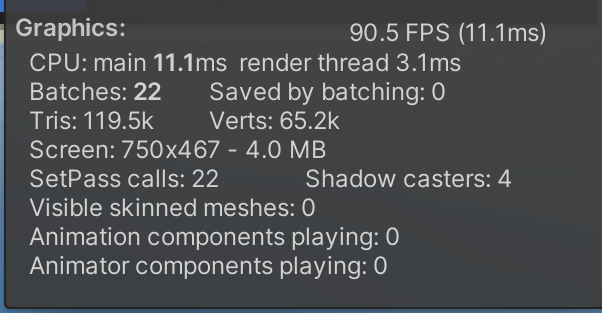
\includegraphics[width=0.6\textwidth]{images/12UAVs_test.png}
    \caption{This is a screenshot from the simulator during a benchmark test with 12 drones and around 30 live AIS vessels. The test was run in Unity Editor on the laptop described above. The simulator was running at around 90 FPS, with CPU idling around 25\%.}
    \label{fig:12UAVs_Unity_benchmark}
\end{figure}
